\clearpage
\setcounter{topnumber}{3}
\setcounter{dbltopnumber}{2}
\setcounter{totalnumber}{4}
\renewcommand{\topfraction}{0.9}
\renewcommand{\dbltopfraction}{0.9}
\renewcommand{\textfraction}{0.1}
\renewcommand{\floatpagefraction}{0.9}
\renewcommand{\dblfloatpagefraction}{0.9}

\section*{Appendix}

\startcontents[appendix]
\printcontents[appendix]{}{1}{\setcounter{tocdepth}{2}}

\vspace{1em}

\section{Prompts}
\label{app:prompts}

This appendix lists the prompts verbatim, with placeholders in typewriter font.
In training, the student receives each problem of DAPO-Math-17k in the user message $\mathcal{P}_{\text{train}}$, and in evaluation, each problem of the benchmarks in $\mathcal{P}_{\text{eval}}$.
In the other prompts, \texttt{\{student prompt\}} stands for the complete user message $\mathcal{P}_{\text{train}}$ of the problem.
The critic is the teacher model.
It receives the solution of the student split into paragraphs at blank lines, where headings, separator lines, and short lead-in lines are merged into the next paragraph, and the prompts call these paragraphs segments.

\begin{prompt}[title={$\mathcal{P}_{\text{eval}}$ --- user message of the student and the teacher in evaluation}]
\texttt{\{problem\}} Please reason step by step, and put your final answer within \verb|\boxed{}|.
\end{prompt}

\subsection{Prompts of \ours{}}
\label{app:prompts-method}

The critic of \ours{} receives the system prompt $\mathcal{P}_{\text{critic}}$, which defines the task and the output format, and the user message $\mathcal{P}_{\text{critic-user}}$, which gives the problem, the reference answer, and the numbered paragraphs of the solution.
For a rollout that reaches the length limit, the first paragraph of $\mathcal{P}_{\text{critic}}$ is replaced by $\mathcal{P}_{\text{critic}}^{\text{len}}$.
From the reply of the critic, we parse the listed errors and build the feedback, which ends with the reference answer.
\ours{} keeps the rollout up to the end of the paragraph of the last listed error and appends $\mathcal{P}_{\text{fb}}$, which contains the feedback.
The student continues after $\mathcal{P}_{\text{fb}}$, and the teacher scores this continuation with $\mathcal{P}_{\text{fb}}$ in its context, whereas the training sequence of the student does not contain $\mathcal{P}_{\text{fb}}$.

\begin{prompt}[title={$\mathcal{P}_{\text{train}}$ --- user message of the student in training (DAPO-Math-17k)}]
Solve the following math problem step by step. The last line of your response should be of the form Answer: \$Answer (without quotes) where \$Answer is the answer to the problem.\\[4pt]
\texttt{\{problem\}}\\[4pt]
Remember to put your answer on its own line after ``Answer:''.
\end{prompt}

\begin{prompt}[title={$\mathcal{P}_{\text{critic}}$ --- system prompt of the critic}]
You are a meticulous math teacher. A student has submitted a complete solution whose FINAL ANSWER IS WRONG. You are given the correct answer. Use it as a reference to trace the student's work forward and find the steps that contain genuine errors.\\[4pt]
How to locate the errors:\\
Read the numbered segments in order. For each one ask: given everything before it, is this step correct? List every segment that contains a genuine error, in the order in which they appear.\\[4pt]
Do NOT flag a segment merely because it is: an exploratory attempt the student later abandons or corrects; a longer route than necessary; or sloppy notation that does not change the mathematics. Flag only a step that is actually wrong.\\[4pt]
Rules you must follow:\\
1. List the erroneous segments in order of appearance.\\
2. For each one, quote verbatim the single sentence that carries the error.\\
3. For each one, say what is wrong and what to do instead. The student will resume writing after the last listed error, so phrase it as guidance they can act on. Two or three sentences per error.\\
4. NEVER reveal the final answer. Do not state it, do not write an expression that evaluates to it, do not say what it should be. Describe the method, not the result.\\
5. If every step looks correct to you and you cannot identify a genuine error, reply with SEGMENT: NONE. Do not guess {-}{-} a wrong location is worse than none.\\[4pt]
Reply in exactly this format, one block per error:\\
ERROR 1\\
SEGMENT: <index>\\
QUOTE: <the exact wrong sentence, copied verbatim>\\
FEEDBACK: <what is wrong and what to do instead>\\
ERROR 2\\
SEGMENT: <index>\\
QUOTE: <...>\\
FEEDBACK: <...>
\end{prompt}

\begin{prompt}[title={$\mathcal{P}_{\text{critic}}^{\text{len}}$ --- first paragraph of $\mathcal{P}_{\text{critic}}$ for a rollout that reaches the length limit}]
You are a meticulous math teacher. A student's solution ran on without ever reaching an answer. You are given the correct answer. Use it as a reference to trace the student's work forward and find the steps that sent the reasoning off track. If the work is still on a valid path and was merely slow, reply SEGMENT: NONE.
\end{prompt}

\begin{prompt}[title={$\mathcal{P}_{\text{critic-user}}$ --- user message of the critic}]
Problem:\\
\texttt{\{student prompt\}}\\[4pt]
Correct answer (reference only {-}{-} never reveal it): \texttt{\{reference answer\}}\\[4pt]
Student's solution, split into numbered segments:\\[4pt]
{[}0{]} \texttt{\{segment 0\}}\\[4pt]
{[}1{]} \texttt{\{segment 1\}}\\[4pt]
\dots
\end{prompt}

\begin{prompt}[title={$\mathcal{P}_{\text{fb}}$ --- text appended to the kept prefix of the rollout}]
\texttt{\{kept prefix\}}\\[4pt]
{[}Teacher feedback{]} \texttt{\{feedback\}}\\[4pt]
Using this feedback, continue the solution from here. Put your final answer in \verb|\boxed{}|.
\end{prompt}

\begin{prompt}[title={\texttt{\{feedback\}} in $\mathcal{P}_{\text{fb}}$ when the critic lists $k > 1$ errors; for $k = 1$, the lines before the last line are only \texttt{\{feedback 1\}}}]
Your solution contains \texttt{\{k\}} errors.\\
(1) In ``\texttt{\{quote 1\}}'': \texttt{\{feedback 1\}}\\
(2) In ``\texttt{\{quote 2\}}'': \texttt{\{feedback 2\}}\\
\dots\\
The correct final answer is \texttt{\{reference answer\}}.
\end{prompt}

Each quote is cut to $200$ characters.

\subsection{Prompts of the Ablations}
\label{app:prompts-ablation}

All variants in Table~\ref{tab:ablation} use the critic of \ours{}.
The variant without the answer omits the last line of the feedback, and its critic removes every listed error whose feedback contains the reference answer while the solution of the student does not.
The variants in (b) and (c) of Table~\ref{tab:ablation} change this variant, and the runs in Appendices~\ref{app:hyper} and~\ref{app:olmo} use the same feedback.
The variant without the critique keeps only the last line of the feedback, which states the reference answer, and the variant with generic feedback replaces the feedback by $\mathcal{P}_{\text{generic}}$.

\begin{prompt}[title={$\mathcal{P}_{\text{generic}}$ --- generic feedback}]
Your solution contains errors. Check the previous reasoning and redo it.
\end{prompt}

\subsection{Prompts of the Diagnosis}
\label{app:prompts-diag}

The diagnosis in Section~\ref{sec:critique-ability} uses the critic of \ours{} without the reference answer.
The first paragraph of $\mathcal{P}_{\text{critic}}$ is replaced by $\mathcal{P}_{\text{critic}}^{\text{diag}}$ for a complete solution and by $\mathcal{P}_{\text{critic}}^{\text{part}}$ for a truncated solution, and the line with the reference answer is removed from $\mathcal{P}_{\text{critic-user}}$.
The judge receives the system prompt $\mathcal{P}_{\text{judge}}$ and the user message $\mathcal{P}_{\text{judge-user}}$, which lists the errors that the critic claims.
The generic hint in Appendix~\ref{app:rewrite-analysis} replaces the feedback in $\mathcal{P}_{\text{fb}}$ by $\mathcal{P}_{\text{hint}}$.

\begin{prompt}[title={$\mathcal{P}_{\text{critic}}^{\text{diag}}$ --- first paragraph of $\mathcal{P}_{\text{critic}}$ in Section~\ref{sec:critique-ability}, complete solution}]
You are a meticulous math teacher. A student has submitted a complete solution whose FINAL ANSWER IS WRONG. Trace the student's work forward and find the steps that contain genuine errors.
\end{prompt}

\begin{prompt}[title={$\mathcal{P}_{\text{critic}}^{\text{part}}$ --- first paragraph of $\mathcal{P}_{\text{critic}}$ in Section~\ref{sec:critique-ability}, truncated solution}]
You are a meticulous math teacher. A student has written part of a solution, and the solution is not finished yet. Trace the student's work forward and find the steps that contain genuine errors. If every step so far is correct, reply SEGMENT: NONE.
\end{prompt}

\begin{prompt}[title={$\mathcal{P}_{\text{judge}}$ --- system prompt of the judge (Qwen3-8B)}]
You are an expert mathematics grader. You are given a math problem, its correct answer, a student's solution split into numbered segments, and a list of errors that a teacher claims to have found in the solution, in order of appearance. For every listed error, decide whether the claim is right.\\[4pt]
Labels:\\
NEW\_ERROR - the flagged step contains a genuine mistake of its own (a wrong formula, wrong logic, an arithmetic slip, a misread condition, an unjustified claim) that would still be wrong even if every earlier step were correct.\\
PROPAGATED - the reasoning in the flagged step is valid in itself; it is wrong only because it uses a value, expression or conclusion produced by an earlier mistake.\\
RESTATEMENT - the flagged step only restates or reports a wrong result that was already reached earlier (for example the final answer line or a summary), with no new reasoning.\\
NOT\_AN\_ERROR - the flagged step is actually correct.\\[4pt]
Reply with exactly one line per listed error and nothing else, in this format:\\
ERROR 1: \textless{}LABEL\textgreater{}\\
ERROR 2: \textless{}LABEL\textgreater{}
\end{prompt}

\begin{prompt}[title={$\mathcal{P}_{\text{judge-user}}$ --- user message of the judge; for a truncated solution, the third line reads ``Student's partial solution (not finished yet), split into numbered segments:''}]
Problem:\\
\texttt{\{student prompt\}}\\[4pt]
Correct answer: \texttt{\{reference answer\}}\\[4pt]
Student's solution, split into numbered segments:\\[4pt]
{[}0{]} \texttt{\{segment 0\}}\\[4pt]
{[}1{]} \texttt{\{segment 1\}}\\[4pt]
\dots\\[4pt]
Errors claimed by the teacher:\\[4pt]
ERROR 1\\
SEGMENT: \texttt{\{index\}}\\
QUOTE: \texttt{\{quote\}}\\
TEACHER'S NOTE: \texttt{\{feedback\}}\\[4pt]
\dots
\end{prompt}

\begin{prompt}[title={$\mathcal{P}_{\text{hint}}$ --- generic hint in Appendix~\ref{app:rewrite-analysis}}]
Your solution contains an error. Check it and continue.
\end{prompt}

\subsection{Prompts of the Baselines}
\label{app:prompts-baselines}

SFT, KD, GRPO, OPD, FastOPD, SKD, and RelayOPD use $\mathcal{P}_{\text{train}}$.
TRD lets the teacher rewrite one solution of the student per prompt with the system prompt $\mathcal{P}_{\text{TRD}}^{\text{sys}}$ and the user message $\mathcal{P}_{\text{TRD}}$.
OPSD-T gives the student $\mathcal{P}_{\text{train}}$ and scores its rollout with a teacher that receives $\mathcal{P}_{\text{OPSD}}$.
Critique-GRPO critiques an incorrect rollout as \ours{} does, including the reference answer at the end of the feedback, and the student then answers again in a new conversation with the system prompt $\mathcal{P}_{\text{CGRPO}}^{\text{sys}}$ and the user message $\mathcal{P}_{\text{CGRPO}}$.

\begin{prompt}[title={$\mathcal{P}_{\text{TRD}}^{\text{sys}}$ --- system prompt of the TRD rewrite}]
Please reason step by step, and put your final answer within \textbackslash{}boxed\{\}.
\end{prompt}

\begin{prompt}[title={$\mathcal{P}_{\text{TRD}}$ --- user message of the TRD rewrite}]
Your task is to rewrite your mathematical solution.\\[4pt]
**Problem:**\\
\texttt{\{student prompt\}}\\[4pt]
**Your Initial Solution:**\\
\texttt{\{initial solution\}}\\[4pt]
**Instructions:**\\
1. Preserve the overall structure and reasoning path of your original solution\\
2. Identify and fix errors in computation or logic\\
3. Keep correct intermediate steps and meaningful work\\
4. Output ONLY the rewritten solution
\end{prompt}

\begin{prompt}[title={$\mathcal{P}_{\text{OPSD}}$ --- user message of the teacher in OPSD-T}]
\texttt{\{student prompt\}}\\[4pt]
{[}Reference answer: \texttt{\{reference answer\}}{]}
\end{prompt}

\begin{prompt}[title={$\mathcal{P}_{\text{CGRPO}}^{\text{sys}}$ --- system prompt of the refinement in Critique-GRPO}]
You are a helpful assistant.
\end{prompt}

\begin{prompt}[title={$\mathcal{P}_{\text{CGRPO}}$ --- user message of the refinement in Critique-GRPO}]
Given the following inputs:\\
**Question**: \texttt{\{student prompt\}}\\
**Previous Solution**: \texttt{\{initial solution\}}\\
**Critique**: \texttt{\{feedback\}}\\[4pt]
Please re-answer by:\\
- Correcting potential errors identified in the critique, if they exist.\\
- Providing clear, step-by-step reasoning.\\
- Formatting the final answer as \verb|`\boxed{answer}`|.\\[4pt]
Ensure the revised solution addresses all issues raised in the critique.
\end{prompt}

\section{Details of the Diagnosis}
\label{app:diagnosis}

\subsection{Rollouts and Cut Points}

The diagnosis uses the Qwen3-1.7B student after $80$ steps of OPD with seed $42$
and the teacher of the main experiments.
The student generates one rollout for each of $900$ problems from
DAPO-Math-17k with temperature $1.0$, top-$p$ $1.0$, and at most $16{,}384$
tokens, and we grade each rollout with the reward function of training.
We randomly select $150$ correct and $150$ incorrect rollouts.
An incorrect rollout must end with a final answer, so we exclude rollouts that
reach the length limit.
We split each response into paragraphs at blank lines, as \ours{} does.
The cut points are the empty prefix and the $7$ paragraph boundaries that lie
closest to the positions $1/8, \dots, 7/8$ of the response.

\subsection{Continuations and Success Rates}

From each cut point, the teacher and the student each generate $16$
continuations of the prefix of the student within the same assistant turn.
Each model uses its own chat template, temperature $1.0$, top-$p$ $1.0$, and a
budget of $16{,}384$ tokens minus the length of the prefix.
$\Lambda^T(h)$ and $\Lambda^S(h)$ are the fractions of correct continuations of
the teacher and the student from the prefix $h$.
A problem is solvable by the teacher if the teacher succeeds in at least $8$ of
the $16$ continuations from the empty prefix.
All bands are $95\%$ bootstrap confidence intervals with $2{,}000$ resamples of
rollouts.

\subsection{Critique and Judgment}

For Figure~\ref{fig:critique}(b), the teacher critiques the truncated solution at
every cut point with $\mathcal{P}_{\text{critic}}^{\text{part}}$
(Appendix~\ref{app:prompts-diag}).
It decodes greedily for at most $2{,}048$ tokens, and we apply the filters of
training.
Qwen3-8B in thinking mode judges every listed error with the reference answer in
its context.
It labels an error as a new mistake, a mistake that follows from an earlier one,
a restatement of an earlier wrong result, or not an error, and we count every
label other than the last as real.
The judge samples with temperature $0.6$, top-$p$ $0.95$, and top-$k$ $20$ and
generates at most $16{,}384$ tokens.

\subsection{Rewrite Analysis}
\label{app:rewrite-analysis}

Figure~\ref{fig:rewrite-effect} uses the incorrect rollouts in which the success
rate of the teacher, estimated from its first $8$ continuations, is at least
$0.5$ at the empty prefix and falls below $0.5$ at a later cut point.
To enlarge this set, we add the $204$ remaining incorrect rollouts from the same
$900$ problems, which gives $163$ such rollouts.
The teacher critiques each complete solution with the prompts of \ours{}, and
$161$ critiques keep at least one error after filtering.
We cut each rollout as \ours{} does and draw $8$ continuations per condition.
At the cut point, the teacher continues with and without the critique, and the
student continues without the critique, with the critique, and with the generic
hint $\mathcal{P}_{\text{hint}}$.
At $25\%$, $50\%$, and $75\%$ of a rewrite that the student writes with the
critique, the teacher continues with the critique and the student continues
without it.
At the same positions of the discarded part of the original rollout, both
continue without the critique.

\subsection{Diagnosis with the Qwen3-0.6B Student}
\label{app:diag-06b}

We repeat the diagnosis with the Qwen3-0.6B student after $40$ steps of OPD
with seed $42$, which is the checkpoint in Table~\ref{tab:main}, and keep the
teacher, the problems, and all other settings.
Of the $900$ rollouts, $270$ are correct, $593$ are incorrect, and $37$ reach the
length limit.
Figures~\ref{fig:failure-region-06b}, \ref{fig:critique-06b}, and
\ref{fig:rewrite-effect-06b} correspond to Figures~\ref{fig:failure-region},
\ref{fig:critique}, and \ref{fig:rewrite-effect}, and they show the same
pattern as the Qwen3-1.7B student.
On the $106$ incorrect rollouts from problems that the teacher solves,
$\Lambda^T$ falls from $0.89$ at the empty prefix to $0.38$ at the last cut
point, and the fraction of teacher continuations that end with the incorrect
answer of the student rises from $0.00$ to $0.15$.
Across the groups of $\Lambda^T$, whose means range from $0.05$ to $0.92$,
between $77\%$ and $84\%$ of the errors that the teacher lists are real.
For Figure~\ref{fig:rewrite-effect-06b}, we add the $443$ remaining incorrect
rollouts as in Appendix~\ref{app:diagnosis}, which gives $304$ rollouts in which
the success rate of the teacher falls below $0.5$, and $295$ critiques keep at
least one error.
After the cut point, the success rate of the teacher falls from $0.45$ to $0.14$
on the original rollout and stays between $0.70$ and $0.75$ on the rewrite, and
the success rate of the student rises from $0.06$ to $0.12$ on the rewrite.

\begin{figure}[t]
\centering
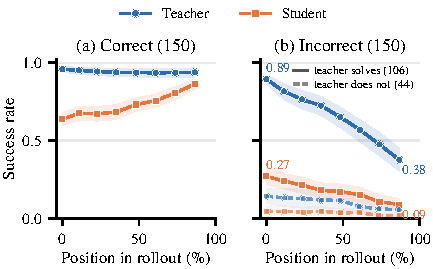
\includegraphics[width=\columnwidth]{figures/fig_failure_region_small.pdf}
\caption{Expected accuracy of the teacher and the Qwen3-0.6B student from prefixes of the student on (a) correct and (b) incorrect rollouts.}
\label{fig:failure-region-06b}
\end{figure}

\begin{figure}[t]
\centering
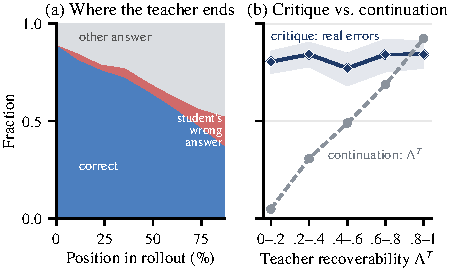
\includegraphics[width=\columnwidth]{figures/fig_critique_small.pdf}
\caption{(a) Outcomes of the continuations of the teacher and (b) fraction of the listed errors that are real, for the Qwen3-0.6B student.}
\label{fig:critique-06b}
\end{figure}

\begin{figure}[t]
\centering
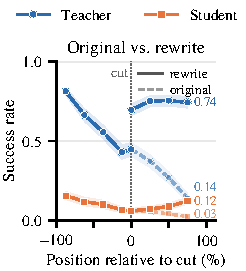
\includegraphics[width=0.58\columnwidth]{figures/fig_rewrite_small.pdf}
\caption{Success rates of the teacher and the Qwen3-0.6B student around the cut point.}
\label{fig:rewrite-effect-06b}
\end{figure}

\subsection{Occupancy Mismatch}
\label{app:occupancy}

\begin{figure*}[t]
\centering
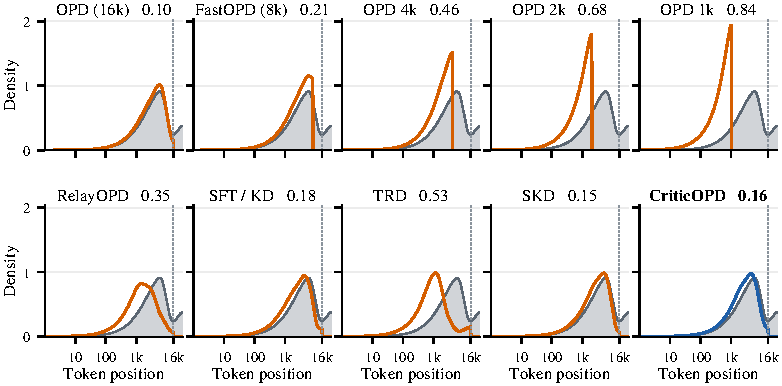
\includegraphics[width=\textwidth]{figures/fig_mismatch_positions.pdf}
\caption{Token positions of the prefixes that each method supervises (colored) and of the inference prefixes (gray), with the total variation distance in each title. The dotted line marks the training limit of $16{,}384$ tokens.}
\label{fig:mismatch-positions}
\end{figure*}

\begin{figure*}[t]
\centering
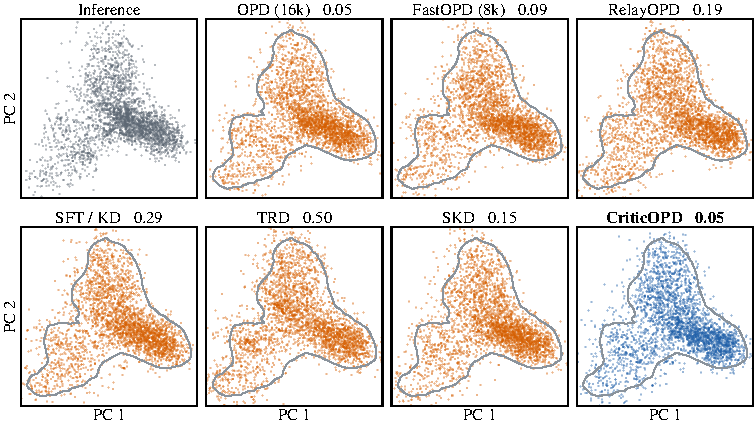
\includegraphics[width=\textwidth]{figures/fig_mismatch_hidden.pdf}
\caption{Hidden states of the student on the prefixes that each method supervises, projected onto the first two principal components of the inference states. The contour encloses $95\%$ of the inference states, and each title gives the classifier bound on the total variation distance.}
\label{fig:mismatch-hidden}
\end{figure*}

The measurement in Section~\ref{sec:experiments-why} uses the first $256$ problems in the training order of DAPO-Math-17k with seed $42$ and the student of Section~\ref{sec:diagnosis}.
For $d_\theta$, the student generates four rollouts per problem with temperature $1.0$, top-$p$ $1.0$, and at most $32{,}768$ tokens, and every generated token contributes one position.
For $d_m$, CriticOPD, RelayOPD, and SKD each run one training step on these problems from the same student, and every token that receives a loss contributes one position.
For OPD, we take all positions of the original rollouts in the step of CriticOPD, which the student generates with the training limit of $16{,}384$ tokens.
FastOPD differs from OPD only in the length limit, so we take the first $8{,}192$ positions of these rollouts, and the first $1{,}024$, $2{,}048$, and $4{,}096$ positions for the shorter limits.
SFT and KD train on the same teacher solutions of these problems, and TRD trains on the solutions that the teacher rewrites from rollouts of the student, so every response token of these data contributes one position.
We split the positions from $1$ to $32{,}768$ into $48$ intervals of equal width on a logarithmic scale and merge the intervals whose rounded boundaries coincide, which leaves $45$ intervals.
We compute the total variation distance between the two position distributions over these intervals.
The curves in Figure~\ref{fig:mismatch-positions} are kernel density estimates over the logarithm of the position and serve only for display.

Figure~\ref{fig:mismatch-positions} shows the position distributions of all methods.
A shorter length limit moves the supervision to earlier positions, and the distance grows from $0.10$ for OPD to $0.21$, $0.46$, $0.68$, and $0.84$ for limits of $8{,}192$, $4{,}096$, $2{,}048$, and $1{,}024$ tokens.
RelayOPD and TRD supervise shorter sequences than the student generates, with distances of $0.35$ and $0.53$.
SFT, KD, and SKD stay close to inference in position, with distances of $0.18$ and $0.15$.
At inference, $9.3\%$ of the tokens lie after position $16{,}384$, which no method with a training limit of $16{,}384$ tokens supervises.

The position does not reflect the content of a prefix, so we also compare the hidden states of the student, which are the inputs to its output layer at the prefixes.
We sample $20{,}000$ states per method and $30{,}000$ states for inference uniformly over tokens, subtract the mean inference state of each problem, and divide each dimension by its standard deviation over the inference states.
A logistic regression separates the states of a method from an equal number of inference states, with five folds that split the problems.
If its held-out accuracy is $a$, then $2a-1$ is a lower bound on the total variation distance between the two state distributions.
Two disjoint halves of the inference rollouts give $-0.02$, which is the noise level.
Figure~\ref{fig:mismatch-hidden} projects the states onto the first two principal components of the inference states.
CriticOPD has a distance of $0.05$, the same as OPD and lower than FastOPD ($0.09$), SKD ($0.15$), and RelayOPD ($0.19$).
SFT and KD ($0.29$) and TRD ($0.50$) train on text that the teacher writes or rewrites and have the largest distances in hidden states, although SFT and KD stay close to inference in position.

\section{Experimental Details}
\label{app:setup}

\subsection{Training}

\begin{table}[h]
\centering
\caption{\textbf{Hyperparameters} of all methods.}
\label{tab:hyper}
\scriptsize
\setlength{\tabcolsep}{4pt}
\renewcommand{\arraystretch}{1.08}
\begin{tabular}{ll}
\toprule
\textbf{Setting} & \textbf{Value} \\
\midrule
\multicolumn{2}{l}{\textit{Training}} \\
Prompts per step & $128$ \\
Rollouts per prompt & $1$ (GRPO: $8$) \\
Optimizer updates per step & $1$ \\
Learning rate & $10^{-6}$, constant, no warmup \\
Maximum prompt length & $2{,}048$ \\
Maximum response length & $16{,}384$ (FastOPD: $8{,}192$) \\
Rollout temperature, top-$p$ & $1.0$, $1.0$ \\
Checkpoint interval & $20$ steps \\
GPUs & $4$ ($2$ student, $2$ teacher) \\
\midrule
\multicolumn{2}{l}{\textit{Critic of \ours{}}} \\
Decoding & greedy \\
Maximum critique length & $2{,}048$ \\
Number of listed errors & all \\
\midrule
\multicolumn{2}{l}{\textit{Evaluation}} \\
Temperature, top-$p$ & $1.0$, $1.0$ \\
Maximum new tokens & $32{,}768$ \\
Samples per problem & $32$ (AIME, AMC), $8$ (others) \\
\bottomrule
\end{tabular}
\end{table}

Table~\ref{tab:hyper} lists the shared hyperparameters.
OPD optimizes the sampled reverse-KL objective of Equation~\eqref{eq:adv} with
the policy gradient and applies no KL penalty.
One epoch over DAPO-Math-17k takes $139$ steps.

\subsection{Software and Hardware}
\label{app:software}

We implement all methods on the code of RelayOPD \citep{xu2026relay}, which
builds on \texttt{verl} 0.9.0.dev \citep{sheng2025hybridflow}, and the released
code fixes the commit of this code base.
The software consists of Python 3.12, PyTorch 2.11 with CUDA 13.0,
Transformers 5.15, and Ray 2.57.
vLLM 0.21 \citep{kwon2023vllm} generates the rollouts and the critiques, and a
separate vLLM server computes the log-probabilities of the teacher on the
training sequences.
We grade mathematical answers with Math-Verify 0.9.0 and code with EvalPlus
0.3.1.
Each training run uses one node with four NVIDIA A100-SXM4-80GB GPUs, two for
the student and two for the teacher.
The seed-$42$ runs of OPD, FastOPD, and RelayOPD on Qwen3-1.7B use four GPUs
for each model with the same batch size, and GRPO and SFT, which use no
teacher during training, use all four GPUs for the student.
Runs on Qwen3-0.6B use A100, H100, H200, or B200 GPUs, and each evaluation job
uses one GPU.

\subsection{Configuration of \ours{}}
\label{app:config}

Algorithm~\ref{alg:criticopd} summarizes one training step of \ours{}.
The critic is the teacher.
If a critique reaches the length limit, we discard its last item, which is
incomplete.
The feedback lists the remaining items and ends with the reference answer
(Appendix~\ref{app:prompts-method}).
Rollouts that reach the response limit are also sent to the critic, with a
prompt that tells the critic the solution is unfinished
(Appendix~\ref{app:prompts-method}).
The rewrite uses the response budget that remains after the kept prefix.
We train \ours{} for $40$ steps on Qwen3-1.7B and for $80$ steps on Qwen3-0.6B,
and select the step as for all methods (Appendix~\ref{app:selection}).

\begin{algorithm}[t]
\caption{CriticOPD Training}
\label{alg:criticopd}
\begin{algorithmic}[1]
\Require Student $\pi_\theta$, teacher $\pi_T$,
batch $\{(x,a)\}$
\State $\mathcal{L}_{\mathrm{ours}} \gets 0$
\For{each $(x,a)$ in the batch}
    \State Sample $y \sim \pi_\theta(\cdot\mid x)$
    \If{$y$ is incorrect or truncated}
        \State Generate critique $c$ using $\pi_T$ given $(x,y,a)$
        \State Discard incomplete error items from $c$
    \EndIf
    \If{a valid critique is available}
        \State $\tau \gets$ first position after the last critiqued paragraph
        \State $\tilde{y}_{<\tau} \gets y_{<\tau}$
        \State Sample $\tilde{y}_{\geq\tau}
        \sim \pi_\theta(\cdot\mid h_\tau,c)$
        \State $\ell \gets \mathcal{L}_{\mathrm{fb}}(\tilde{y};c)$
    \Else
        \State $\ell \gets \mathcal{L}_{\mathrm{OPD}}(y)$
    \EndIf
    \State $\mathcal{L}_{\mathrm{ours}}
    \gets \mathcal{L}_{\mathrm{ours}}+\ell$
\EndFor
\State Update $\theta$ using $\mathcal{L}_{\mathrm{ours}}$
\end{algorithmic}
\end{algorithm}

\begin{figure*}[t]
\centering
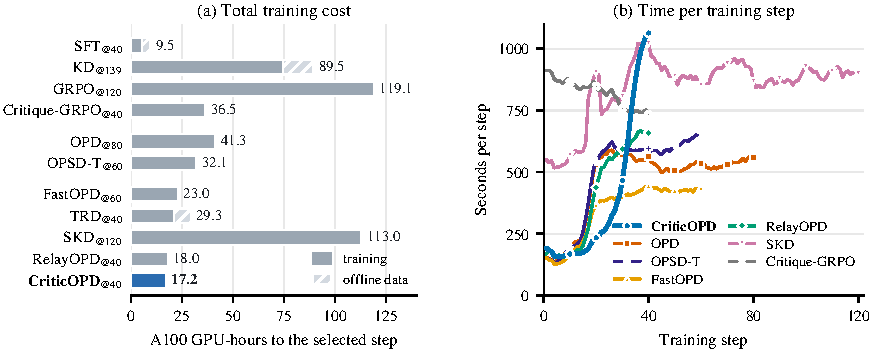
\includegraphics[width=\textwidth]{figures/fig_cost.pdf}
\caption{Training cost of the Qwen3-1.7B students. (a) A100 GPU-hours until the
selected step, including the generation of offline data. (b) Seconds per
training step, averaged over five steps.}
\label{fig:cost}
\end{figure*}

\subsection{Baselines}

SFT trains the student with cross-entropy on one solution of the teacher per
prompt, which the teacher samples with temperature $1.0$ and which we do not
filter by correctness.
KD trains on the same solutions with the forward KL divergence on the $128$
most probable tokens of the teacher.
GRPO uses a binary correctness reward and no teacher.
FastOPD is OPD with a maximum response length of $8{,}192$ tokens during
training.
TRD lets the teacher rewrite one solution of the student per prompt and fix its
errors, and it trains the student on the rewrites with the objective of KD.
SKD generates rollouts by speculative decoding: the teacher accepts a draft
token of the student if the token is among its $5$ most probable tokens and
otherwise samples a replacement, and the student is trained with the objective
of KD.
RelayOPD lets the teacher take over for at most $3$ paragraphs or $256$ tokens
when the teacher predicts a reflection token that is outside the $5$ most
probable tokens of the student.
It allows at most two takeovers, ends the rollout after the second one, and
applies the OPD objective to all tokens.
OPSD-T trains as OPD, except that the teacher scores each rollout with the
reference answer after the problem ($\mathcal{P}_{\text{OPSD}}$ in
Appendix~\ref{app:prompts-baselines}).
The student generates and is trained without the reference answer, and no
rollout is critiqued or rewritten.
Critique-GRPO follows its official implementation and uses only the outcome
reward.
The student samples $7$ rollouts per prompt.
If all of them are incorrect, the critic of \ours{} critiques each of them with
the feedback ending with the reference answer, and the student answers again in
a new conversation with $\mathcal{P}_{\text{CGRPO}}$.
One of these refinements, a correct one if any, joins the group as an eighth
response.
The advantage is the reward minus the mean reward of the group, without the
normalization by the standard deviation that GRPO uses.
Tokens of the initial rollouts use the importance ratio without clipping, the
tokens of the refinement are weighted by $p/(p+0.1)$, where $p$ is their
probability under the student, and the entropy coefficient is $0.001$.

\subsection{Evaluation}

The benchmarks contain $30$ (AIME 2024), $30$ (AIME 2025), $83$ (AMC 2023),
$500$ (MATH500), $675$ (OlympiadBench), and $272$ (Minerva Math) problems.
The students generate in non-thinking mode, and Avg is the macro average over
the six benchmarks.
For each method, we select one step with seed $42$
(Appendix~\ref{app:selection}), train seeds $43$ and $44$ to the same step, and
report the mean and the sample standard deviation over the three seeds.
The teacher and the initial students are evaluated once.

\subsection{Checkpoint Selection}
\label{app:selection}

We select checkpoints on a validation set that does not overlap with the
training data or the six test benchmarks.
We call a problem contaminated if at least half of its $13$-grams appear in
DAPO-Math-17k or in a test benchmark, or if its normalized text equals that of
such a problem.
A single shared $13$-gram is not enough, because common phrases such as ``where
$m$ and $n$ are relatively prime positive integers. Find $m+n$'' already contain
more than $13$ words.
The validation set has two parts.
MATH-val starts from the $4{,}500$ test problems of MATH outside MATH500, of
which $1{,}304$ are contaminated, $1{,}284$ of them by DAPO-Math-17k, and we
sample $500$ of the remaining $3{,}196$ problems uniformly with seed $0$.
Comp-val contains all $153$ problems of four competitions from 2025 in MathArena
\citep{balunovic2025matharena}, namely BRUMO, CMIMC, HMMT February, and SMT, and
none of them is contaminated.
We do not use AIME 2022 and 2023, because $54$ of their $60$ problems appear in
DAPO-Math-17k.
The validation set uses the prompt $\mathcal{P}_{\text{eval}}$, the chat
template, the stop tokens, the grader, and the sampling parameters of the test
benchmarks, with up to $32{,}768$ new tokens, and it draws $4$ samples per
problem on MATH-val and $8$ on Comp-val.
The accuracy of each part averages the fraction of correct samples over its
problems, and the validation score is the mean of the accuracies of the two
parts.

The candidates of each method are the checkpoints at every multiple of $20$
steps and at the last step of training if it is not a multiple of $20$.
We select the candidate with the highest validation score, and the earlier step
if two candidates tie.
For Qwen3-1.7B and Qwen3-0.6B, we select once for each student and method with
the checkpoints of seed $42$ and use the selected step for all seeds.
For the OLMo-3 student, we make no selection and reuse the steps selected for
Qwen3-1.7B, with the exceptions that Appendix~\ref{app:olmo} describes.
The test results do not enter the selection.

\begin{table*}[t]
\centering
\caption{
\textbf{Results with OLMo-3 models} on six mathematical reasoning benchmarks with seed $42$.
The subscript after each method gives the step, and bold marks the best student.
}
\label{tab:olmo}

\scriptsize
\setlength{\tabcolsep}{3pt}
\renewcommand{\arraystretch}{1.05}

\begin{tabularx}{\textwidth}{l*{7}{>{\centering\arraybackslash}X}}
\toprule
\textbf{Method}
& \textbf{AIME24}
& \textbf{AIME25}
& \textbf{AMC23}
& \textbf{MATH500}
& \textbf{OlympiadBench}
& \textbf{Minerva}
& \textbf{Avg}
\\
\midrule

Teacher
& 73.54 & 60.62 & 92.24 & 96.22 & 77.35 & 47.43
& 74.57 \\

\midrule
\multicolumn{8}{c}{\textit{Student: Olmo-3-7B-Instruct-SFT, teacher: Olmo-3.1-32B-Instruct}} \\
\midrule

Student
& 6.15 & 4.17 & 30.50 & 64.80 & 30.09 & 29.09
& 27.47 \\

\arrayrulecolor{black!35}\specialrule{0.35pt}{1.2pt}{1.2pt}\arrayrulecolor{black}

SFT$_{@40}$
& 31.56 & 26.15 & 59.45 & 79.50 & 51.91 & 31.66
& 46.70 \\

KD$_{@80}$
& 35.42 & 30.83 & 72.33 & 86.83 & 59.48 & 33.27
& 53.03 \\

GRPO$_{@120}$
& 10.00 & 7.60 & 37.46 & 69.85 & 36.28 & 30.70
& 31.98 \\

Critique-GRPO$_{@40}$
& 6.56 & 4.90 & 31.40 & 65.67 & 31.15 & 29.32
& 28.17 \\

\arrayrulecolor{black!35}\specialrule{0.35pt}{1.2pt}{1.2pt}\arrayrulecolor{black}

OPD$_{@60}$
& 41.04 & 31.98 & 71.54 & 87.58 & 60.61 & 35.39
& 54.69 \\

OPSD-T$_{@60}$
& 41.46 & 34.90 & 72.29 & 88.40 & 61.80 & 34.42
& 55.54 \\

\arrayrulecolor{black!35}\specialrule{0.35pt}{1.2pt}{1.2pt}\arrayrulecolor{black}

FastOPD$_{@60}$
& 38.23 & 33.33 & 71.05 & 88.05 & 60.65 & 35.52
& 54.47 \\

TRD$_{@40}$
& 27.50 & 24.48 & 56.25 & 79.55 & 50.70 & 31.66
& 45.02 \\

SKD$_{@60}$
& 38.82 & 29.33 & 70.82 & 86.61 & 59.30 & 33.78
& 53.11 \\

RelayOPD$_{@40}$
& 32.60 & 27.08 & 67.47 & 84.67 & 57.22 & 33.55
& 50.43 \\

\rowcolor{blue!8}
\textbf{\ours{}}$_{@60}$
& \textbf{43.44} & \textbf{37.81} & \textbf{74.70}
& \textbf{89.08} & \textbf{62.33} & \textbf{36.02}
& \textbf{57.23} \\

\rowcolor{blue!8}
\textcolor{green!50!black}{$\Delta$ vs OPD}
& \textcolor{green!50!black}{+2.40}
& \textcolor{green!50!black}{+5.83}
& \textcolor{green!50!black}{+3.16}
& \textcolor{green!50!black}{+1.50}
& \textcolor{green!50!black}{+1.72}
& \textcolor{green!50!black}{+0.63}
& \textcolor{green!50!black}{+2.54} \\

\bottomrule
\end{tabularx}
\end{table*}

\section{Computational Cost}
\label{app:cost}

Figure~\ref{fig:cost} compares the training cost of all methods on the
Qwen3-1.7B student.
We measure the time of every training step under seeds $43$ and $44$, in which
all methods run on four A100 GPUs, and average the two seeds.
For SFT, KD, and TRD, we add the time to generate the offline data on A100 GPUs.
The time per step of \ours{} grows from about $170$ seconds over the first $10$
steps to about $870$ seconds over steps $31$ to $40$, compared with $160$ and
$560$ seconds for OPD, because the responses of the student grow longer and
incorrect rollouts receive a critique and a rewrite.
Over the same $40$ steps, \ours{} uses $0.96$ times the GPU-hours of OPD.
\ours{} reaches its selected step after $40$ steps, so its total cost of
$17.2$ GPU-hours is $0.42$ times that of OPD at step $80$.
GRPO and Critique-GRPO, which sample $8$ rollouts per prompt, take about $890$
and $820$ seconds per step.

\begin{table*}[t]
\centering
\caption{
\textbf{Results outside mathematics} for Qwen3-1.7B. Code uses EvalPlus
pass@1 on the extended tests.
}
\label{tab:ood}

\scriptsize
\setlength{\tabcolsep}{3pt}
\renewcommand{\arraystretch}{1.05}

\begin{tabularx}{\textwidth}{l*{7}{>{\centering\arraybackslash}X}}
\toprule
\textbf{Method}
& \textbf{MMLU-Pro}
& \textbf{MMLU}
& \textbf{ARC-C}
& \textbf{OpenBookQA}
& \textbf{HumanEval+}
& \textbf{MBPP+}
& \textbf{Avg}
\\
\midrule

Teacher
& 69.75 & 80.09 & 94.94 & 93.95 & 82.00 & 74.70
& 82.57 \\

Student
& 38.10 & 55.24 & 77.69 & 74.10 & 62.50 & 56.50
& 60.69 \\

\midrule

SFT
& 50.80 & 63.29 & 84.41 & 79.70 & 63.10 & 55.40
& 66.12 \\
KD
& 50.85 & 63.78 & 84.28 & 79.30 & 64.00 & 57.10
& 66.55 \\
GRPO
& 51.41 & 61.49 & 81.68 & 78.75 & 63.70 & 58.50
& 65.92 \\
\arrayrulecolor{black!35}\specialrule{0.35pt}{1.2pt}{1.2pt}\arrayrulecolor{black}
OPD
& 56.61 & 67.14 & 87.07 & 83.80 & 66.30 & 61.90
& 70.47 \\
\arrayrulecolor{black!35}\specialrule{0.35pt}{1.2pt}{1.2pt}\arrayrulecolor{black}
FastOPD
& 56.14 & 66.27 & 85.52 & 83.40 & 66.50 & 61.20
& 69.84 \\
TRD
& 47.44 & 61.22 & 81.08 & 75.45 & 62.80 & 57.20
& 64.20 \\
SKD
& 53.84 & 65.87 & 85.90 & 81.65 & 63.70 & 59.90
& 68.48 \\
RelayOPD
& 56.04 & 66.40 & 85.90 & 83.20 & 66.90 & 60.40
& 69.81 \\
\rowcolor{blue!8}
\textbf{\ours{}}
& 57.31 & 67.88 & 87.73 & 84.90 & 65.90 & 60.40
& 70.69 \\

\bottomrule
\end{tabularx}
\end{table*}

\section{Additional Results}
\label{app:results}

\subsection{Results with OLMo-3 Models}
\label{app:olmo}

Table~\ref{tab:olmo} repeats the comparison with models from another family.
The student is Olmo-3-7B-Instruct-SFT, and the teacher is Olmo-3.1-32B-Instruct, which shares the tokenizer of the student.
All methods use the training recipe and the evaluation protocol of Table~\ref{tab:main} with seed $42$.
Each method is trained to the step selected for Qwen3-1.7B, except that OPD and \ours{} are both evaluated at step $60$, and that we stop KD and SKD early, at steps $80$ and $60$ instead of $139$ and $120$.
The critique of \ours{} here does not end with the reference answer.
\ours{} raises the average of OPD from $54.69$ to $57.23$.
As with the Qwen3 students, the gains are largest on the competition benchmarks, with $+5.83$ on AIME 2025 and $+3.16$ on AMC 2023.

\begin{table*}[t]
\centering
\caption{\textbf{Per-benchmark results of the ablations} on Qwen3-1.7B with
seed $42$. The rows follow Table~\ref{tab:ablation}.}
\label{tab:ablation-full}
\scriptsize
\setlength{\tabcolsep}{3pt}
\renewcommand{\arraystretch}{1.05}
\begin{tabularx}{\textwidth}{l *{7}{>{\centering\arraybackslash}X}}
\toprule
\textbf{Variant} & \textbf{AIME24} & \textbf{AIME25} & \textbf{AMC23} & \textbf{MATH500} & \textbf{Olympiad} & \textbf{Minerva} & \textbf{Avg} \\
\midrule
\rowcolor{blue!8}
\ours{} & 40.52 & 29.06 & 70.18 & 89.40 & 60.59 & 37.64 & 54.57 \\
\midrule
\multicolumn{8}{@{}l}{\textit{(a) Content of the feedback}} \\
\quad \textit{w/o} answer & 41.56 & 27.60 & 67.43 & 88.75 & 59.04 & 37.91 & 53.72 \\
\quad \textit{w/o} critique & 34.48 & 21.96 & 60.33 & 85.55 & 54.83 & 34.89 & 48.67 \\
\quad critique + answer $\rightarrow$ generic & 40.00 & 27.71 & 67.39 & 88.05 & 58.91 & 36.63 & 53.11 \\
\midrule
\multicolumn{8}{@{}l}{\textit{(b) Writer of the suffix}} \\
\quad student $\rightarrow$ teacher & 38.12 & 28.23 & 68.45 & 87.48 & 59.37 & 36.72 & 53.06 \\
\midrule
\multicolumn{8}{@{}l}{\textit{(c) Scoring of the suffix}} \\
\quad \textit{w/o} feedback & 38.85 & 27.19 & 67.09 & 87.72 & 58.41 & 35.94 & 52.53 \\
\midrule
OPD & 34.69 & 22.71 & 63.33 & 86.70 & 56.31 & 37.32 & 50.18 \\
\bottomrule
\end{tabularx}
\end{table*}

\subsection{Results Outside Mathematics}
\label{app:ood}

Table~\ref{tab:ood} reports the results of the Qwen3-1.7B students outside mathematics.
We evaluate on MMLU-Pro, MMLU, ARC-Challenge, OpenBookQA, HumanEval+, and MBPP+
with $4$ samples per problem and a budget of $32{,}768$ tokens.
For MMLU and MMLU-Pro, we use subsets of $2{,}000$ questions that keep the
proportion of each subject.
We grade multiple-choice answers by the option letter in the final box and
report EvalPlus pass@1 on the extended tests for code.

\subsection{Per-Benchmark Ablation Results}
\label{app:ablation}

Table~\ref{tab:ablation-full} reports the six benchmarks for every variant in
Table~\ref{tab:ablation}, all at step $40$ except OPD at step $80$.

\subsection{Sensitivity to Hyperparameters}
\label{app:hyper}

\ours{} adds two hyperparameters to OPD: the number $k$ of listed errors that
the feedback contains, and the length limit of the critique.
The rewrite starts after the $k$-th error.
Figure~\ref{fig:hyper} varies each hyperparameter and keeps the other at its
default, which uses all listed errors and a limit of $2{,}048$ tokens.
The average rises with $k$, from $51.56$ with one error to $53.31$ with three
and $53.72$ with all errors, so the feedback on later errors still helps.
The length limit matters until most critiques fit: limits of $512$ and
$1{,}024$ tokens cut off $79\%$ and $27\%$ of the critiques and give $51.72$
and $52.78$, whereas limits of $2{,}048$ and $4{,}096$ tokens cut off $6\%$ and
$3\%$ and give similar averages ($53.72$ and $53.31$).

\begin{figure}[H]
\centering
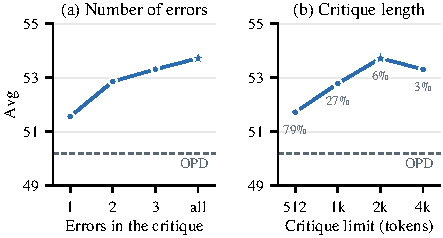
\includegraphics[width=\columnwidth]{figures/fig_hyper.pdf}
\caption{Sensitivity of \ours{} on the Qwen3-1.7B student with seed $42$. The
star marks the default, and the numbers in (b) give the share of truncated
critiques.}
\label{fig:hyper}
\end{figure}

\begin{figure*}[t]
\centering
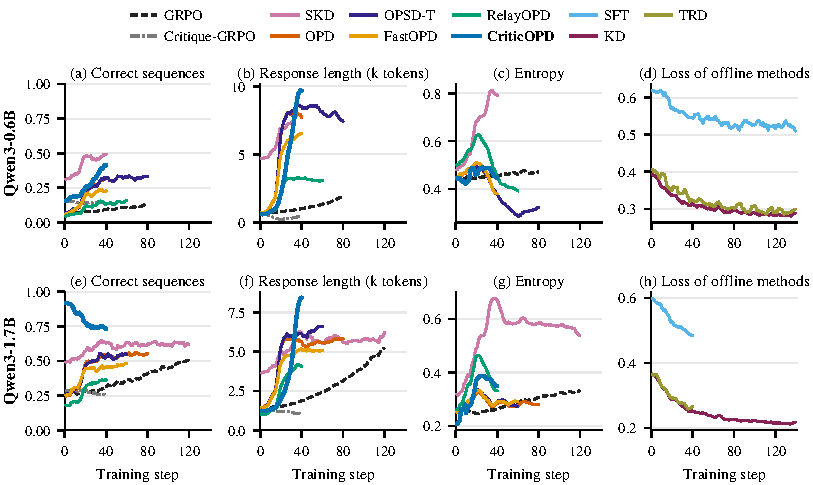
\includegraphics[width=\textwidth]{figures/fig_dynamics.pdf}
\caption{Training dynamics, averaged over seeds and smoothed over five steps.}
\label{fig:dynamics}
\end{figure*}

\subsection{Training Dynamics}
\label{app:dynamics}

Figure~\ref{fig:dynamics} shows the training dynamics of all methods.
Panels (a) and (e) report the fraction of training sequences that reach the
reference answer.
These sequences contain the tokens that the teacher samples in SKD, the
takeovers of the teacher in RelayOPD, the refinements in Critique-GRPO, and the
rewrites after the critique in \ours{}, so this fraction is not the accuracy of
the student alone.
The entropy of Critique-GRPO is not shown, because its loss sums over the tokens
and divides by a constant length, so its logged entropy is not a mean over
tokens.
Panels (d) and (h) report the training loss of the methods that train on
offline data, which is the cross-entropy for SFT and the forward KL divergence
for KD and TRD.
The training logs of seed $42$ are missing for SFT, KD, and TRD on Qwen3-0.6B,
so these curves average seeds $43$ and $44$.
At both scales, the training sequences of \ours{} become longer than those of
OPD, which agrees with the longer responses at evaluation
(Section~\ref{sec:experiments-why}).

\subsection{Generation Length}
\label{app:budget}

The student of \ours{} writes longer responses than the student of OPD, with
$10.2$k tokens per response on average, compared with $5.3$k.
Figure~\ref{fig:budget} evaluates the Qwen3-1.7B students under generation
budgets from $4$k to $32$k tokens.
We reuse the responses with the budget of $32{,}768$ tokens and count a response
as incorrect if it is longer than the budget.
\ours{} falls below OPD at $4$k and $8$k tokens and exceeds it at $16$k and
$32$k.

\begin{figure}[!t]
\centering
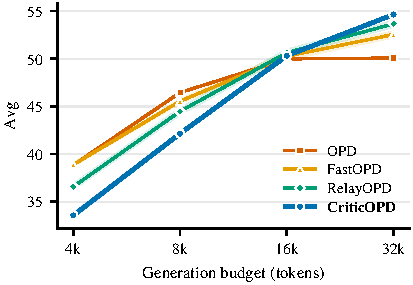
\includegraphics[width=\columnwidth]{figures/fig_budget.pdf}
\caption{Average over six benchmarks when responses longer than the budget
count as incorrect, over three seeds of Qwen3-1.7B.}
\label{fig:budget}
\end{figure}

\begin{table}[!t]
\centering
\caption{\textbf{Length-controlled comparison} on Qwen3-1.7B, averaged over
three seeds.}
\label{tab:length}
\footnotesize
\setlength{\tabcolsep}{4pt}
\begin{tabular}{@{}lccc@{}}
\toprule
\textbf{Method} & \textbf{AIME length} & \textbf{Avg@16k} & \textbf{Avg@32k} \\
\midrule
OPD & $8{,}487$ & 49.99 & 50.08 \\
FastOPD & $11{,}910$ & 50.27 & 52.55 \\
\midrule
\rowcolor{blue!8}
\ours{} & $12{,}457$ & 50.32 & 54.65 \\
\quad scoring \textit{w/o} feedback & $12{,}065$ & 50.62 & 52.26 \\
\quad critique $\rightarrow$ generic & $12{,}051$ & 50.86 & 52.87 \\
\bottomrule
\end{tabular}
\end{table}

Longer responses alone do not explain the gain.
Table~\ref{tab:length} compares variants that share the rewriting of \ours{} and
produce responses of about the same median length on AIME.
At the 32k generation budget, when the teacher scores the rewrite without the critique, the average is
$2.39$ points lower than that of \ours{} with the same feedback, and generic
feedback lowers it by $1.78$ points.
FastOPD also writes responses of a similar length and is $2.10$ point lower.
At the same response length, the critique in the context of the teacher
therefore still improves the student.
